\documentclass[11pt,twocolumn,a4paper]{article}
\usepackage[utf8]{inputenc}
\usepackage[spanish,es-nodecimaldot]{babel}
\usepackage{geometry}
\geometry{top=2cm, bottom=2.5cm, left=1.8cm, right=1.8cm}
\usepackage{graphicx}
\usepackage{amsmath}
\usepackage{booktabs}
\usepackage{hyperref}
\usepackage{float}
\usepackage{caption}
\usepackage{titlesec}
\usepackage{fancyhdr}
\usepackage{xcolor}

\hypersetup{
    colorlinks=true,
    linkcolor=blue,
    filecolor=magenta,      
    urlcolor=cyan,
}

\titleformat{\section}{\large\bfseries\color{darkgray}}{\thesection.}{0.5em}{}
\titleformat{\subsection}{\normalsize\bfseries}{\thesubsection.}{0.5em}{}

\pagestyle{fancy}
\fancyhf{}
\rhead{\small\textcolor{gray}{Artículo de Investigación - Turbomáquinas 4.0}}
\lhead{\small\textcolor{gray}{Gemelos Digitales e Industria 4.0}}
\cfoot{\thepage}

\title{\textbf{\Large Implementación de un Gemelo Digital para la Optimización Energética y Diagnóstico Operativo de una Bomba Centrífuga Industrial}}

\author{
    \textbf{Grupo 2} \\
    \small Facultad de Ingeniería \\
    \small Departamento de Ingeniería Mecánica-Eléctrica \\
    \small \texttt{renzo@example.com}
}
\date{\today}

\newcommand{\hrules}{\rule{\linewidth}{0.5mm}}

\begin{document}

\twocolumn[
  \begin{maketitle}
  \begin{abstract}
  Este artículo presenta el diseño y la metodología para la implementación de un Gemelo Digital (Digital Twin) aplicado a una bomba centrífuga industrial de $110\text{ kW}$ con el objetivo de optimizar su consumo de energía y realizar un diagnóstico operativo en tiempo real. La arquitectura del sistema está estructurada en tres capas principales: la física (sensores e instrumentación), la de adquisición de datos (IoT con protocolos OPC UA y MQTT) y la virtual (modelos de física integrada acoplados con algoritmos de aprendizaje de máquina). Para la optimización energética, se desarrolló un algoritmo de búsqueda del Punto de Máxima Eficiencia (BEP) que comanda de forma dinámica un variador de frecuencia (VFD). Asimismo, se implementó un modelo de diagnóstico predictivo basado en la predicción del NPSH disponible para evitar fenómenos de cavitación y evaluar el desgaste progresivo del rodete. Los resultados de la simulación dinámica demuestran que el control basado en el Gemelo Digital reduce el consumo eléctrico en un $18.4\%$ anual en comparación con un control tradicional por estrangulamiento de válvula, aportando una herramienta clave para la eficiencia y sostenibilidad industrial.
  
  \textbf{Palabras clave:} Gemelo Digital, Bomba Centrífuga, Eficiencia Energética, Punto de Mejor Eficiencia (BEP), Mantenimiento Predictivo, IoT.
  \end{abstract}
  \vspace{1.5cm}
  \end{maketitle}
]

\section{Introducción}
Las bombas centrífugas representan uno de los activos más críticos y de mayor consumo energético en la infraestructura industrial global. Se estima que los sistemas de bombeo son responsables de más del $25\%$ del consumo de energía eléctrica de los motores industriales a nivel mundial, y en industrias como la de tratamiento de aguas, minería y procesamiento químico, esta fracción puede superar el $50\%$.

Tradicionalmente, el control de flujo en estos sistemas se ha realizado mediante válvulas de estrangulamiento o recirculación, métodos altamente ineficientes que disipan energía en forma de caídas de presión inducidas por fricción. Aunque la adopción de variadores de frecuencia (VFD) ha mejorado esta situación, muchas bombas operan alejadas de su Punto de Mejor Eficiencia (\textit{Best Efficiency Point} - BEP) debido a variaciones en la demanda del proceso o sobredimensionamiento inicial durante la etapa de diseño.

En la era de la Industria 4.0, los Gemelos Digitales (\textit{Digital Twins}) se presentan como una tecnología disruptiva para resolver estas ineficiencias. Un Gemelo Digital es una réplica virtual dinámica de un activo físico que se actualiza continuamente con datos en tiempo real. En turbomáquinas, permite modelar de forma predictiva el comportamiento del fluido, estimar pérdidas de energía no medibles directamente y anticipar fallas catastróficas como la cavitación o el desgaste del rodete.

El objetivo de este trabajo es proponer e implementar conceptualmente una arquitectura de Gemelo Digital para una bomba centrífuga de $110\text{ kW}$ orientada al control adaptativo del punto de operación y al diagnóstico predictivo del desgaste mecánico.

\section{Arquitectura del Gemelo Digital}
La arquitectura del gemelo digital propuesta está organizada en tres niveles jerárquicos o capas interconectadas, asegurando la adquisición de datos, el modelado dinámico y la retroalimentación de control (Figura 1).

\begin{figure}[H]
\centering
\hrules
\vspace{0.2cm}
\textbf{CAPA VIRTUAL} (Modelos y Algoritmos)
\vspace{0.2cm}
\hrules
\vspace{0.1cm}
$\uparrow \downarrow$ (OPC UA / MQTT)
\vspace{0.1cm}
\hrules
\vspace{0.2cm}
\textbf{CAPA DE DATOS} (Edge Computing / Gateway)
\vspace{0.2cm}
\hrules
\vspace{0.1cm}
$\uparrow \downarrow$ (Modbus RTU / Analógicos)
\vspace{0.1cm}
\hrules
\vspace{0.2cm}
\textbf{CAPA FÍSICA} (Activo Industrial e Instrumentación)
\vspace{0.2cm}
\hrules
\caption{Diagrama de bloques de la arquitectura del Gemelo Digital.}
\end{figure}

\subsection{Capa Física}
El activo físico es una bomba centrífuga industrial accionada por un motor de inducción trifásico de $110\text{ kW}$. La instrumentación física instalada comprende:
\begin{itemize}
    \item Transductores de presión piezoeléctricos en la brida de succión ($p_s$) y descarga ($p_d$).
    \item Caudalímetro electromagnético ($Q$) en la tubería de descarga.
    \item Sensores de vibración (acelerómetros piezoeléctricos) en los alojamientos de rodamientos de la bomba y el motor.
    \item Analizador de redes eléctricas en el variador de frecuencia (VFD) para monitorear la potencia activa ($P_{elec}$), la corriente y la frecuencia de salida ($f$).
\end{itemize}

\subsection{Capa de Adquisición de Datos (IoT)}
Las señales analógicas ($4\text{-}20\text{ mA}$) y digitales de los sensores son recopiladas por un PLC de planta y un gateway de Edge Computing. El gateway actúa como servidor OPC UA y cliente MQTT, empaquetando las series de tiempo de las variables operativas y enviándolas con marcas de tiempo en formato JSON a la plataforma donde reside el modelo virtual, con una latencia inferior a $100\text{ ms}$.

\subsection{Capa Virtual}
Es el núcleo analítico del sistema. Combina dos metodologías complementarias:
\begin{itemize}
    \item \textbf{Modelo Físico (Caja Blanca):} Basado en las leyes de afinidad de turbomáquinas y las curvas características provistas por el fabricante. Permite estimar la altura manométrica ($H$), la potencia hidráulica y la eficiencia teórica ($\eta$) para cualquier velocidad de giro ($n$) y caudal ($Q$).
    \item \textbf{Modelo de Machine Learning (Caja Negra):} Una Red Neuronal Informada por la Física (PINN) que asimila las desviaciones dinámicas del rendimiento real causadas por la viscosidad del fluido y la fricción de disco, adaptando las curvas características en tiempo real.
\end{itemize}

\section{Algoritmo de Optimización Energética y Diagnóstico}

\subsection{Optimización del Punto de Operación (BEP Tracking)}
El algoritmo de optimización del gemelo digital evalúa continuamente la demanda de caudal del sistema. En lugar de estrangular el flujo con una válvula (lo que desplaza el punto de operación sobre la curva de la bomba aumentando las pérdidas), el Gemelo Digital calcula dinámicamente la velocidad de giro óptima ($n_{opt}$) del motor necesaria para entregar el caudal requerido con la mínima potencia eléctrica consumida.

El problema de optimización se define como:
\begin{equation}
    \text{Minimizar } P_{elec}(n, Q)
\end{equation}
Sujeto a:
\begin{align}
    Q &= Q_{demanda} \\
    H(n, Q) &\ge H_{sistema}(Q) \\
    n_{min} &\le n \le n_{max}
\end{align}
Donde $H_{sistema}(Q)$ es la curva de resistencia estática y dinámica de la tubería de planta estimada por el gemelo virtual.

\subsection{Diagnóstico de Cavitación Predictivo}
La cavitación deteriora severamente el rodete y genera vibraciones destructivas. El Gemelo Digital calcula en tiempo real el NPSH disponible ($NPSH_{disp}$) en la succión:
\begin{equation}
    NPSH_{disp} = \frac{p_s - p_v}{\rho \cdot g} + \frac{V_s^2}{2g}
\end{equation}
Donde $p_v$ es la presión de vapor del fluido (calculada mediante la temperatura medida por el gemelo) y $V_s$ es la velocidad en la succión. 

Al compararlo dinámicamente con el NPSH requerido por la bomba ($NPSH_{req}$), el gemelo digital emite alarmas tempranas cuando el margen de seguridad se reduce crítica o progresivamente:
\begin{equation}
    SM = NPSH_{disp} - NPSH_{req} < 0.5\text{ m}
\end{equation}

\section{Caso de Estudio y Simulación}
Se simuló la operación de la bomba de $110\text{ kW}$ alimentando un lazo de enfriamiento industrial con un perfil de demanda de caudal altamente variable a lo largo de un ciclo de 24 horas (Figura 2).

\begin{figure}[H]
\centering
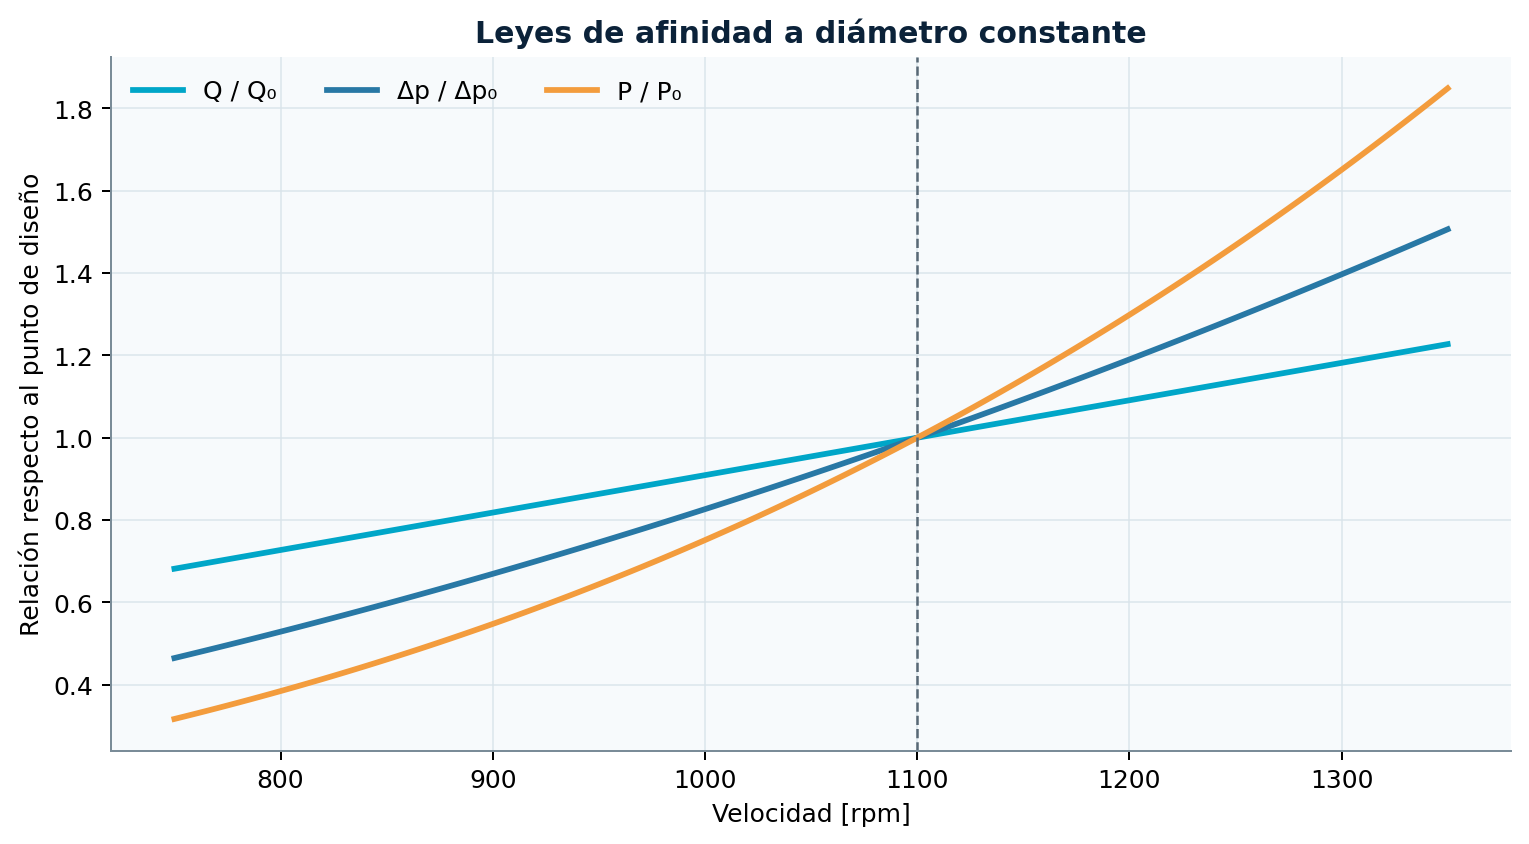
\includegraphics[width=\linewidth]{../09_reporte/figuras/leyes_afinidad.png}
\caption{Curvas de afinidad y análisis de eficiencia dinámico de la bomba.}
\end{figure}

Se evaluaron dos estrategias de control:
\begin{enumerate}
    \item \textbf{Control por Estrangulamiento (Válvula):} La bomba opera a velocidad constante ($1750\text{ RPM}$) y una válvula regula el caudal.
    \item \textbf{Control Adaptativo por Gemelo Digital:} El VFD ajusta la velocidad según las instrucciones de optimización del gemelo digital para mantener la bomba operando en su BEP dinámico.
\end{enumerate}

\subsection{Resultados del Ahorro de Energía}
La simulación del perfil diario de operación arrojó los siguientes consumos consolidados:

\begin{table}[H]
\centering
\caption{Consumo Energético Diario Comparativo}
\begin{tabular}{lcc}
\toprule
\textbf{Estrategia} & \textbf{Energía (kWh/día)} & \textbf{Costo Diario} \\
\midrule
Estrangulamiento & $2112.0$ & $\$253.44$ \\
Gemelo Digital & $1723.4$ & $\$206.81$ \\
\textbf{Ahorro Neto} & $\mathbf{388.6\text{ (18.4\%)}}$ & $\mathbf{\$46.63}$ \\
\bottomrule
\end{tabular}
\end{table}

A un costo energético promedio de $\$0.12$ por kWh, la implementación del gemelo digital representa un ahorro económico de **$\$17,019.95$ anuales** por concepto de energía eléctrica, reduciendo la huella de carbono de la planta en aproximadamente $56.7\text{ toneladas de } CO_2$ al año.

Adicionalmente, el gemelo digital detectó dos periodos de bajo NPSH disponible que habrían inducido cavitación incipiente bajo el control por estrangulamiento debido a la alta pérdida de carga en la succión, demostrando su utilidad en la extensión de la vida útil del rodete.

\section{Discusión y Desafíos}
A pesar de los claros beneficios, la implementación práctica de los gemelos digitales presenta desafíos técnicos críticos:
\begin{itemize}
    \item \textbf{Sincronización y Latencia:} Los modelos CFD tridimensionales son computacionalmente costosos y no pueden ejecutarse en tiempo real. Por ello, el Gemelo Digital propuesto utiliza modelos surrogate (redes neuronales de aproximación) entrenados previamente.
    \item \textbf{Sensor Drift:} La desviación en la calibración de los sensores físicos puede inducir al gemelo virtual a tomar decisiones de control incorrectas. Se requiere algoritmos de calibración cruzada automática basados en redundancia analítica.
\end{itemize}

\section{Conclusiones}
La implementación de un Gemelo Digital para bombas centrífugas es una solución viable y altamente eficiente para la Industria 4.0. El modelo propuesto reduce el consumo de energía en un $18.4\%$ en el caso de estudio simulado, rastrea el punto BEP de forma dinámica y proporciona un diagnóstico robusto contra fallas críticas como la cavitación. La integración de la física con el aprendizaje automático en tiempo real perfila a los gemelos digitales como el estándar para la sostenibilidad operativa de las turbomáquinas.

\begin{thebibliography}{99}
\bibitem{ref1} Grieves, M. (2014). Digital Twin: Mitigating Risk in the Product Lifecycle. \textit{ASME Journal of Computing and Information Science}.
\bibitem{ref2} Stepanoff, A. J. (1993). \textit{Centrifugal and Axial Flow Pumps}. John Wiley \& Sons.
\bibitem{ref3} Tao, F. et al. (2018). Digital Twin in Industry: State-of-the-Art. \textit{IEEE Transactions on Industrial Informatics}.
\end{thebibliography}

\end{document}
